\documentclass[a4paper,12pt]{article}
\usepackage[english,polish]{babel}
\usepackage{polski}
\usepackage[utf8]{inputenc}
\usepackage{graphicx}
\usepackage{array}
\newcommand{\HRule}{\rule{\linewidth}{0.5mm}}

\setlength\fboxsep{1pt}
\setlength\fboxrule{0pt}
\def \tscale {0.3}

\begin{document}
\begin{titlepage}
	\begin{center}
		
\includegraphics[width=0.4\textwidth]{data/logo.jpg} \\[1cm]
		\textsc{\LARGE Technika Mikroprocesorowa} \\[0.8cm]
		\HRule \\[0.4cm]
		{ \huge \bfseries Gesture Processing Library - Projekt} \\[0.4cm] %touch to dotyk;)
		\HRule \\[1.5cm]
	\end{center}
	\begin{minipage}{0.4\textwidth}
		\begin{flushleft} \large
		\emph{Autorzy:} \\
		Michał \textsc{Janiec} \\
		Bartosz \textsc{Polnik}
		\end{flushleft}
	\end{minipage}
\end{titlepage}
\thispagestyle{empty}



\section{\Large Temat} \ \\[0.1cm]
\indent Stworzenie niskopoziomowej biblioteki do przetwarzania gestów, dedykowanej dla mikroprocesorów jedno-układowych.

\section{\Large Cel} \ \\[0.1cm]
\indent Celem projektu jest przede wszystkim stworzenie ww. biblioteki pozwalającej na wygodne korzystanie z technologi multi-touch na różnorodnych urządzeniach. Ponadto utworzona zostanie aplikacja na platformę Android służąca zaprezentowaniu działania biblioteki. Będzie to klon klasycznej gry Tetris.

\section{\Large Opis zagadnienia} \ \\[0.1cm]
\indent Biblioteka zostanie zbudowana zgodnie ze wzorcem fasady. Dla użytkownika zostaną wystawione gesty na dwóch poziomach abstrakcji. Niższy poziom będzie zawierał dokładne informacje o geście w danej chwili. Drugi poziom jedynie binarną informację o wykonaniu jakiegoś gestu. Przykładowo: można wyobrazić sobie prostą przeglądarkę zdjęć. Przłączanie na kolejne zdjęcie można zaimplementować na dwa sposoby: Zdjęcie "śledzi" palec i po przekroczeniu pewnej granicy "nadjeżdża" kolejne, lub rozwiązanie oszczędniejsze w którym zmiana zdjęć nie jest animowana. Widać że dla pierwszego rozwiązania potrzebne są dokładne ruchy, natomiast dla drugiego wystarczy binarna informacja.

\section{\Large Lista gestów} \ \\[0.1cm]
\indent W celu uniknięcia niejednoznaczności proponujemy anglojęzyczne nazwy gestów.\\

\begin{tabular}{|>{\bf}p{2cm}|c|p{4cm}|p{2.5cm}|p{2.5cm}|}
	\hline	\multicolumn{3}{|c}{ }& \multicolumn{2}{|p{5cm}|}{\textbf{Parametry}} \\ \hline
	\textbf{Nazwa}&\textbf{Rysunek}&\textbf{Opis}&\textbf{Uproszczone}&\textbf{Pełne}\\ \hline 
	
     Tap & \fbox{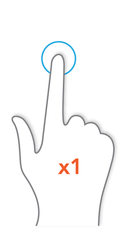
\includegraphics[scale=\tscale]{data/Tap.png}} & 
		Pojedyncze stuknięcie w multi-touch. & 
		Pozycja (x,y)  & Pozycja (x,y) \\ \hline
		
	 Double Tap & \fbox{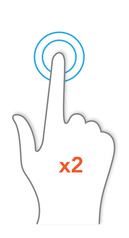
\includegraphics[scale=\tscale]{data/Double_Tap.png}} & 
	 	Szybkie podwójne stuknięcie w multi-touch. & 
	 	Pozycja (x,y) & Pozycja (x,y) \\ \hline
	 	
	 Press & \fbox{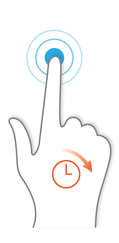
\includegraphics[scale=\tscale]{data/Press.png}} &
	 	Stuknięcie i przytrzymanie palca przez dłuższy czas. & 
	 	Pozycja(x,y) & Pozycja (x,y), Czas \\ \hline
	 	
	 Move & \fbox{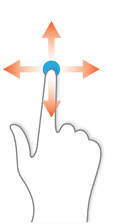
\includegraphics[scale=\tscale]{data/Move}} &
	 	Przesunięcie palca w dowolnym kierunku. & 
	 	Up/Down/ Left/Right & Względne Przesunięcie(x,y), Pozycja(x,y) \\ \hline
	 	
	 Rotate & \fbox{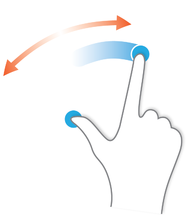
\includegraphics[scale=\tscale]{data/Rotate}} &
	 	Obrót w lewo lub w prawo. & 
	 	Left/Right & Obrót (liczba), Pozycja(x,y) \\ \hline
	 
	 Flick & \fbox{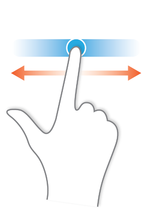
\includegraphics[scale=\tscale]{data/Flick}} &
	 	Przesunięcie palca w lewo lub prawo i puszczenie. &
	 	Left/Right & Przesunięcie względne(x,y), Pozycja(x,y) \\ \hline
	 	
\end{tabular}

\begin{tabular}{|>{\bf}p{2cm}|c|p{4cm}|p{2.5cm}|p{2.5cm}|}
	\hline	\multicolumn{3}{|c}{ }& \multicolumn{2}{|p{5cm}|}{\textbf{Parametry}} \\ \hline
	\textbf{Nazwa}&\textbf{Rysunek}&\textbf{Opis}&\textbf{Uproszczone}&\textbf{Pełne}\\ \hline 

	 Scroll & \fbox{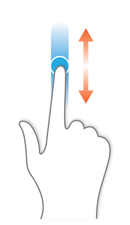
\includegraphics[scale=\tscale]{data/Scroll}} &
	 	Przesunięcie palca w górę lub w dół i puszczenie. &
	 	Up/Down & Przesunięcie względne(x,y), Pozycja(x,y) \\ \hline
	 
	 Zoom & \fbox{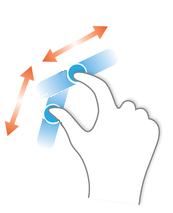
\includegraphics[scale=\tscale]{data/Zoom}} &
	 	Przybliżenie palca wskazującego i kciuka do siebie. &
	 	In/Out & Względne przemieszczenie(x,y) \\ \hline
	 
	 Two Finger Scroll & \fbox{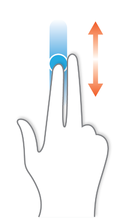
\includegraphics[scale=\tscale]{data/Two_Finger_Scroll}} &
	 	Przesunięcie dwóch palców równolegle w górę lub w dół. &
	 	Up/Down.& Względne przemieszczenie(x,y) Środek miejsca między palcami (x,y) \\ \hline
		
\end{tabular}

\section{\Large Lista wymagań dla biblioteki}
	\subsection*{a) Wymagania Niefunkcjonalne}
	\begin{itemize}
		\item Platforma docelowa - Dowolny mikroprocesor jedno-układowy.
		\item Oszczędność pamięci.
		\item Nie korzystanie z koprocesora.
		\item Optymalność algorytmiczna.
	\end{itemize}
   		
	\subsection*{b) Wymagania Funkcjonalne}
	\begin{itemize}
		\item Rozpoznawanie gestów z powyższej listy.
		\item Wystawianie eventów (zdarzeń) na dwóch poziomach abstrakcji.
		\item Łatwość konfiguracji.
	\end{itemize}

\section{\Large Aplikacja testowa}
Idea gry będzie podobna do tej, znanej nam z Tetris'a. Nowe elementy będą pojawiać się w stałych odstępach czasu, celem użytkownika będzie takie ustawienie elementów, aby możliwie najwięcej ich zmieściło się na ekranie. Przewidujemy również możliwość ich obrotu względem z góry założonego punktu. W momencie wypełnienia przez użytkownika całego rządu elementami, otrzyma on z góry ustaloną ilość punktów, oraz wspomniany rząd zostanie wyczyszczony z elementów (elementy znajdujące się nad nim będą przesunięte o jeden rząd). Będzie to skutkowało wzrostem ilości miejsca na nowe elementy. Dodatkowym sposobem zdobywania punktów będzie czas, przez jaki możliwe będzie pojawianie się nowych elementów na ekranie.

\section{\Large Lista wymagań dla gry}
	\subsection*{a) Wymagania Niefunkcjonalne}
	\begin{itemize}
		\item Platforma docelowa - Android
		\item Różnorodność pojawiających się elementów.
		\item Stworzenie zestawu testów.
	\end{itemize}
   		
	\subsection*{b) Wymagania Funkcjonalne}
	\begin{itemize}
		\item Możliwość przesuwania elementów będą przy pomocy touchpad'a.
		\item Informacja o czasie gry.
		\item Zliczanie punktów zdobytych przez gracza.
		\item Istnienie rankingu umożliwiającego porównanie rezultatów.
	\end{itemize}
	
\section{\Large Wstępny Harmonogram}
\begin{tabular}{l p{10cm}}
	\textsc{Data} & \textsc{Podsumowanie} \\[0.1cm]
	 29.10.2012   &  Określenie harmonogramu prac oraz zakresu projektu\\[0.1cm]
	 19.11.2012   &  Wstępny prototyp umożliwiający wczytanie oraz przetworzenie jednego gestu\\[0.1cm]
	 03.12.2012   &  Wstępny prototyp umożliwiający wczytanie oraz przetworzenie wielu gestów\\[0.1cm] 
	 17.12.2012   &  Działająca wersja aplikacji umożliwiająca wczytanie, przetworzenie oraz interpretację gestów w formie widzialnej dla użytkownika\\[0.1cm]
	 07.01.2013   &  Oddanie działającej biblioteki
\end{tabular}
\end{document}